\documentclass[tikz,border=5pt]{standalone}
\usepackage{luatexja}
\usepackage[hiragino-pron]{luatexja-preset}
\usepackage{amsmath,amssymb}
\usetikzlibrary{arrows.meta,patterns}

\begin{document}
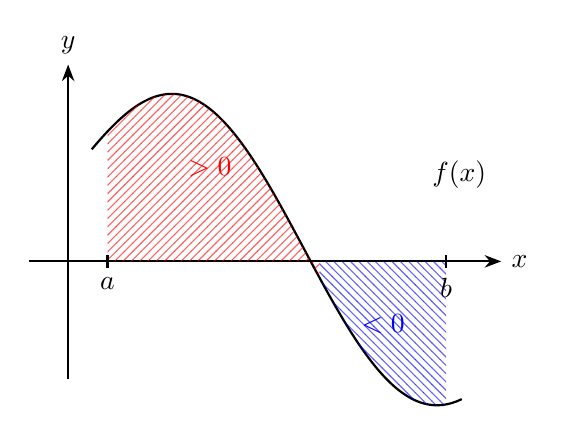
\begin{tikzpicture}

% Axes
\draw[-{Stealth[length=6pt]}, thick] (-0.5,0) -- (5.5,0) node[right] {$x$};
\draw[-{Stealth[length=6pt]}, thick] (0,-1.5) -- (0,2.5) node[above] {$y$};

% f(x) curve
\draw[thick, domain=0.3:5, samples=80, smooth]
  plot (\x, {1.5*sin(60*\x) - 0.3*(\x-2.5) + 0.3});

% Positive region (hatching)
\fill[pattern=north east lines, pattern color=red, opacity=0.6]
  (0.5,0) -- plot[domain=0.5:3.2, samples=60, smooth]
  (\x, {1.5*sin(60*\x) - 0.3*(\x-2.5) + 0.3}) -- (3.2,0) -- cycle;

% Negative region (hatching)
\fill[pattern=north west lines, pattern color=blue, opacity=0.6]
  (3.2,0) -- plot[domain=3.2:4.8, samples=60, smooth]
  (\x, {1.5*sin(60*\x) - 0.3*(\x-2.5) + 0.3}) -- (4.8,0) -- cycle;

% Labels
\node[red] at (1.8,1.2) {$>0$};
\node[blue] at (4.0,-0.8) {$<0$};
\node[above right] at (4.5,0.8) {$f(x)$};

% Boundary marks
\draw[thick] (0.5,0.08) -- (0.5,-0.08) node[below] {$a$};
\draw[thick] (4.8,0.08) -- (4.8,-0.08) node[below] {$b$};

\end{tikzpicture}
\end{document}
